\chapter[Multi-Case Results and Discussion]
{Multi-Case Results\\and Discussion}
\label{ch:results_discussion}

The nominal, hot and cold transient solutions are compared using the common
thermal model defined in Chapter~\ref{ch:thermal_model}. Geometry, nodal
hierarchy, materials and thermal couplings remain unchanged, while the
radiative environment and internal dissipations vary between cases. The
common output-time vector permits a direct comparison throughout the complete
simulated interval.

Absolute curves preserve the temperature, power, heat-flow and energy levels
of each solution. The \textit{Case difference} representation is added when a
direct subtraction provides a clearer measure of the separation from the
nominal case. The electrical conversion and battery model retain the inputs
defined in Chapter~\ref{ch:electrical_battery_analysis}; consequently, their
variations originate from the imported thermal results and the case-dependent
load profiles.


\section{Cases and Comparison Criteria}
\label{sec:comparison_criteria}

The three simulations correspond to the cases listed in
Table~\ref{tab:transient_cases}. The hot case combines greater external heat
input, higher internal dissipations and a shorter eclipse. The cold case
applies lower external input, reduced dissipations and a longer eclipse. No
heater operation is included. The same groups, attributes, source--target
ordering and units are retained whenever the cases are superposed.

For a result $x(t)$, the difference between the nominal case $N$ and a
comparison case $j$ is defined as
\begin{equation}
    \Delta x_{N-j}(t)
    =
    x_N(t)-x_j(t),
    \qquad
    j\in\{H,C\},
    \label{eq:results_case_difference}
\end{equation}
where $H$ and $C$ denote the hot and cold cases. A negative value of
$\Delta x_{N-H}$ therefore indicates that the hot-case result exceeds the
nominal value. This convention is retained in every plot and table generated
with \textit{Case difference}. Absolute curves are preferred when the
operating level is relevant, whereas differences are used to quantify the
separation between solutions or to expose changes hidden by overlapping
curves.


\section{Thermal Response}
\label{sec:thermal_results_comparison}

Applied loads establish the heating and cooling intervals, while the resulting
temperatures determine spatial differences, interface gradients and heat
exchanges.


\subsection{Applied Loads and Temperatures}
\label{subsec:loads_temperature_comparison}

Figure~\ref{fig:solar_panel_load_temperature_comparison} combines the
direct-solar load and mean temperature of \texttt{SOLAR\_PANEL\_1}. The hot
case receives the largest solar input and remains illuminated until the late
part of the simulation. Its eclipse covers only approximately the interval
from $84$ to $96\,\mathrm{min}$. The nominal eclipse extends from about $25$
to $56\,\mathrm{min}$, while the cold case remains without direct solar input
from approximately $42$ to $77\,\mathrm{min}$.

\begin{figure}[H]
    \centering
    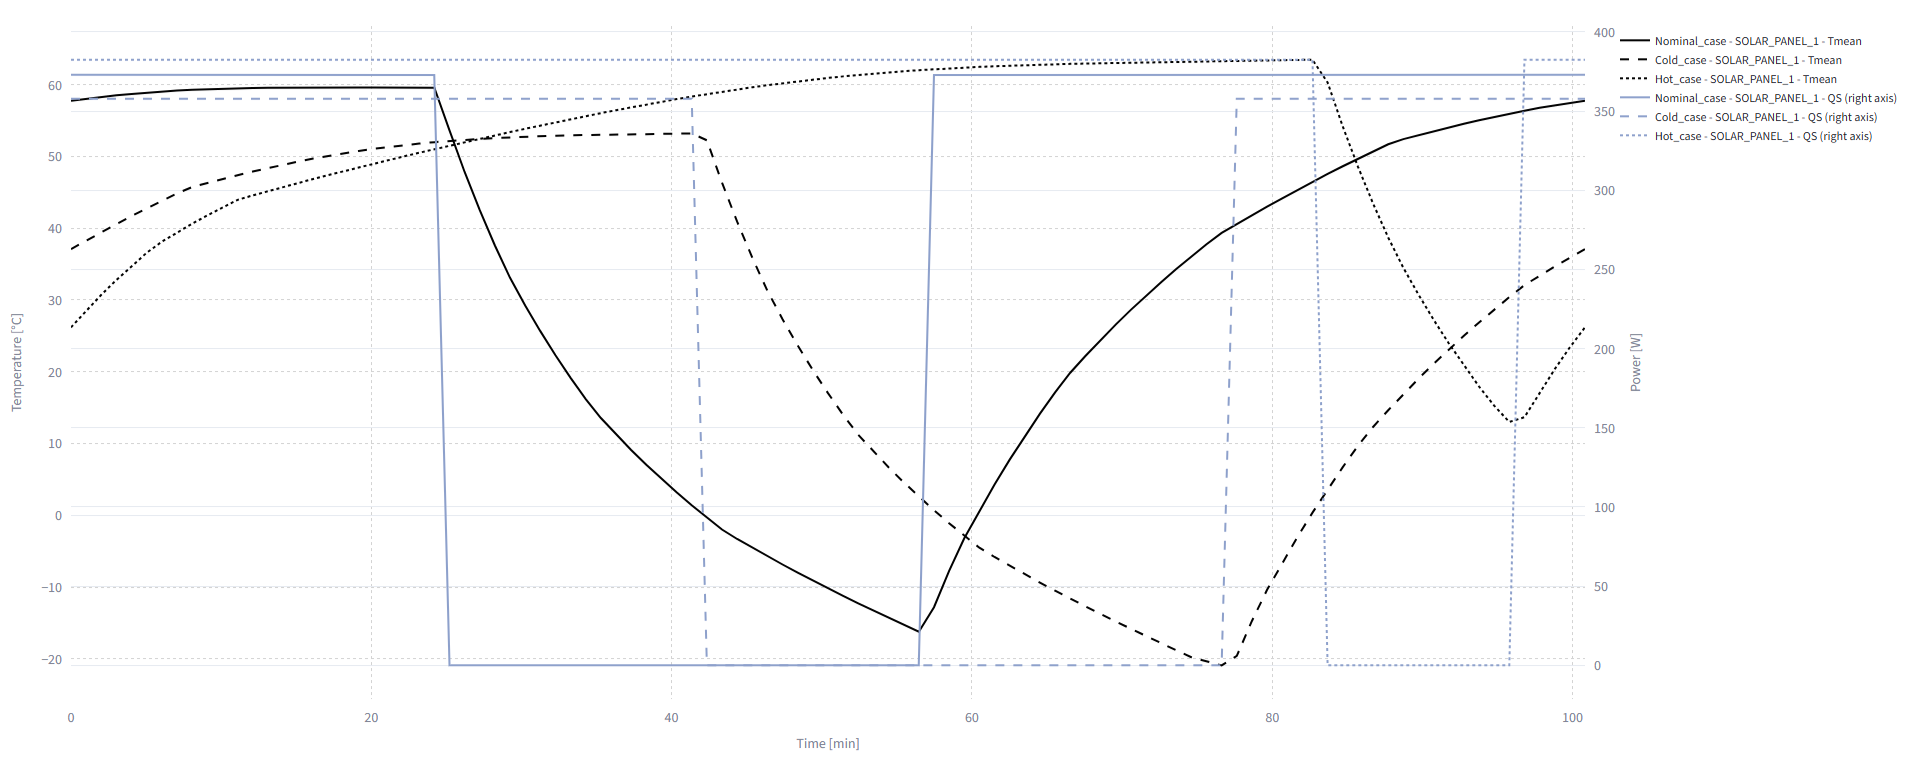
\includegraphics[
        width=1.0\textwidth,
        keepaspectratio
    ]{Figures/09/solar_panel_load_temperature_comparison.png}
    \caption{Direct-solar thermal load and mean temperature of
    \texttt{SOLAR\_PANEL\_1} in the nominal, hot and cold cases.}
    \label{fig:solar_panel_load_temperature_comparison}
\end{figure}

The panel temperature follows the illumination sequence with a delayed
response during each transition. The hot case reaches the highest nodal
temperature, $65.42\,^{\circ}\mathrm{C}$, and remains above
$12.15\,^{\circ}\mathrm{C}$ because of its short eclipse. The nominal and
cold cases cool to $-17.25\,^{\circ}\mathrm{C}$ and
$-21.31\,^{\circ}\mathrm{C}$, respectively. The maximum spatial range inside
\texttt{SOLAR\_PANEL\_1} increases from $5.78\,^{\circ}\mathrm{C}$ in the
hot case to $8.52\,^{\circ}\mathrm{C}$ in the nominal case and
$10.14\,^{\circ}\mathrm{C}$ in the cold case. The lower overall temperature
of the cold solution is therefore accompanied by the largest internal
non-uniformity of the selected panel group.

The internal battery dissipation and mean temperature are compared in
Figure~\ref{fig:battery_load_temperature_comparison}. The prescribed load is
largest in the hot case and smallest in the cold case, both inside and outside
eclipse. The temperature response preserves the same ordering throughout the
simulation: the hot battery remains near $36$--$38\,^{\circ}\mathrm{C}$, the
nominal battery near $18$--$21\,^{\circ}\mathrm{C}$ and the cold battery near
$4\,^{\circ}\mathrm{C}$.

\begin{figure}[H]
    \centering
    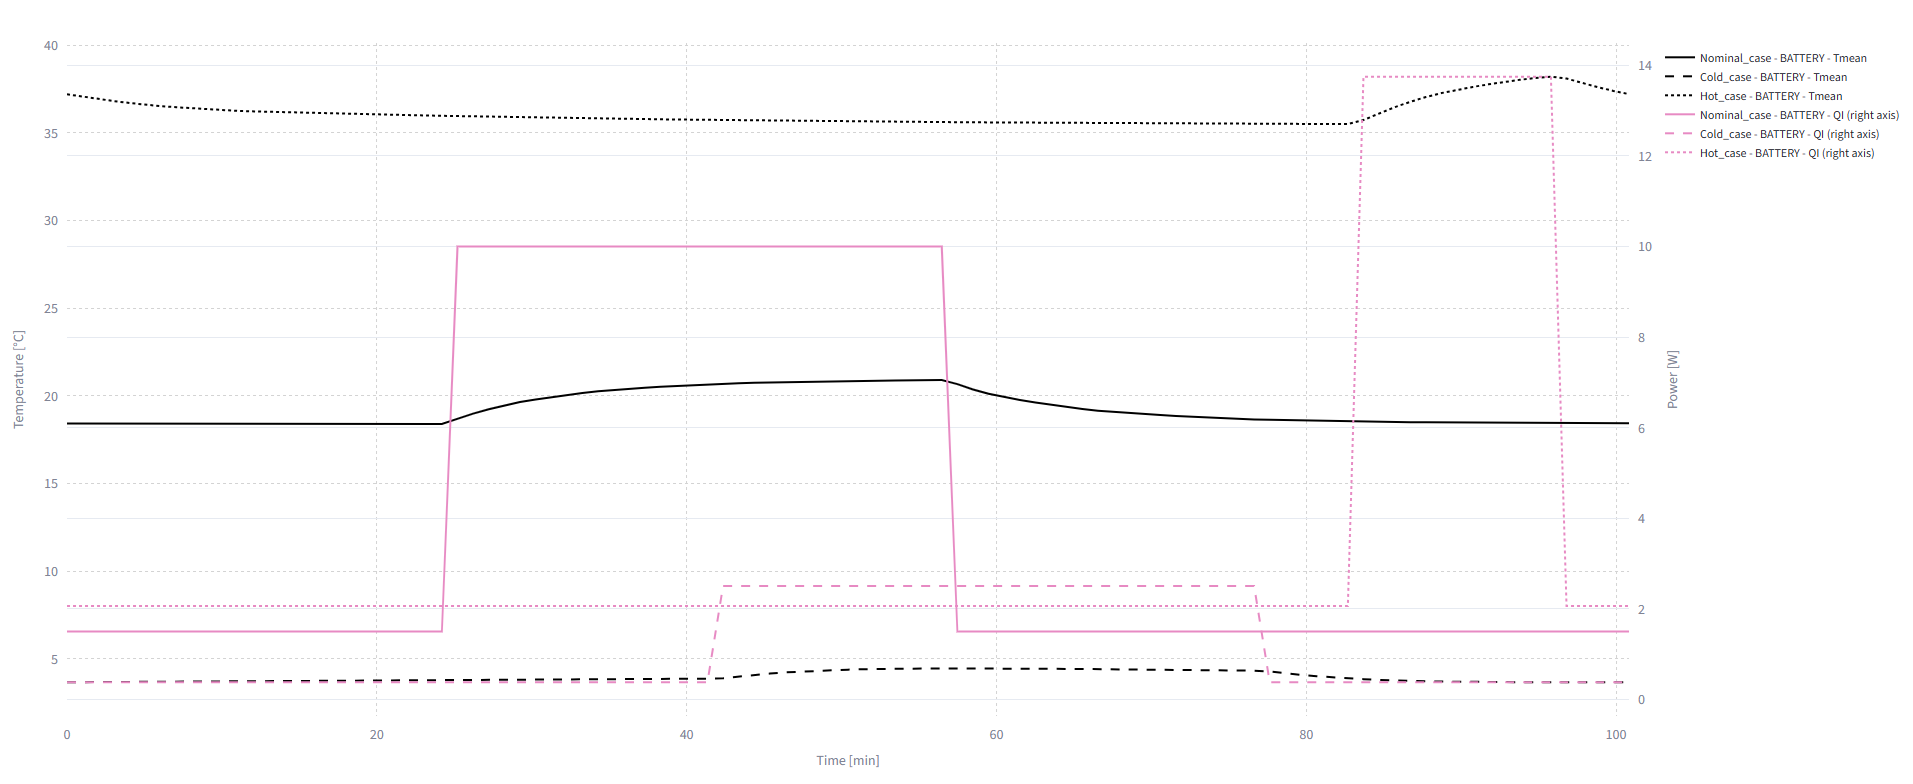
\includegraphics[
        width=0.9\textwidth,
        keepaspectratio
    ]{Figures/09/battery_load_temperature_comparison.png}
    \caption{Internal heat load and mean temperature of \texttt{BATTERY} in
    the three transient cases.}
    \label{fig:battery_load_temperature_comparison}
\end{figure}

The nodal extrema in Table~\ref{tab:multicase_thermal_summary} confirm the
general displacement of the thermal response. The hot case produces the
highest temperatures for all selected elements, whereas the cold case
produces the lowest. The shift is particularly clear in the battery, OBC and
radiator. Battery temperatures range from $35.43$ to
$38.97\,^{\circ}\mathrm{C}$ in the hot case, from $18.25$ to
$21.77\,^{\circ}\mathrm{C}$ in the nominal case and from $3.50$ to
$4.60\,^{\circ}\mathrm{C}$ in the cold case. The radiator follows the same
trend but remains substantially colder, reaching minima of
$5.56\,^{\circ}\mathrm{C}$, $-7.37\,^{\circ}\mathrm{C}$ and
$-17.26\,^{\circ}\mathrm{C}$, respectively.

% File: Tables/table_multicase_thermal_summary.tex
% Usage: \MultiCaseThermalSummaryTable[0.82\textwidth]
% Values obtained from the thermal-summary exports for the nominal, hot and
% cold transient cases.

\newcommand{\MultiCaseThermalSummaryTable}[1][0.82\textwidth]{%
\begin{table}[H]
    \centering
    \caption{Temperature extrema and maximum spatial temperature ranges of
    the selected elements in the nominal, hot and cold transient cases.}
    \label{tab:multicase_thermal_summary}
    \footnotesize
    \renewcommand{\arraystretch}{1.16}
    \setlength{\tabcolsep}{5.0pt}
    \resizebox{#1}{!}{%
    \begin{tabular}{|l|l|c|c|c|}
        \hline
        \textbf{Element} &
        \textbf{Case} &
        \textbf{$T_{\max}$ [$^\circ$C]} &
        \textbf{$T_{\min}$ [$^\circ$C]} &
        \textbf{$\Delta T_{\max}^{\mathrm{sp}}$ [$^\circ$C]} \\ \hline

        \texttt{SOLAR\_PANEL\_1} & Nominal & 62.45 & -17.25 & 8.52 \\ \cline{2-5}
        & Hot  & 65.42 & 12.15  & 5.78 \\ \cline{2-5}
        & Cold & 56.63 & -21.31 & 10.14 \\ \hline

        \texttt{BODY\_PANEL} & Nominal & 18.87 & 5.05  & 13.63 \\ \cline{2-5}
        & Hot  & 35.76 & 20.90 & 14.72 \\ \cline{2-5}
        & Cold & 5.63  & -5.55 & 10.99 \\ \hline

        \texttt{OBC\_BOX} & Nominal & 13.74 & 11.30 & 2.36 \\ \cline{2-5}
        & Hot  & 30.43 & 27.83 & 2.59 \\ \cline{2-5}
        & Cold & 0.85  & -1.28 & 2.05 \\ \hline

        \texttt{RADIATOR} & Nominal & 0.05   & -7.37  & 5.66 \\ \cline{2-5}
        & Hot  & 14.49  & 5.56   & 6.68 \\ \cline{2-5}
        & Cold & -10.85 & -17.26 & 4.88 \\ \hline

        \texttt{BATTERY} & Nominal & 21.77 & 18.25 & 2.98 \\ \cline{2-5}
        & Hot  & 38.97 & 35.43 & 2.90 \\ \cline{2-5}
        & Cold & 4.60  & 3.50  & 0.84 \\ \hline
    \end{tabular}%
    }
\end{table}%
}

\MultiCaseThermalSummaryTable[0.62\textwidth]

The absolute temperature levels do not determine the spatial ranges by
themselves. The hot \texttt{BODY\_PANEL} reaches the largest internal range,
$14.72\,^{\circ}\mathrm{C}$, but the cold battery presents the smallest
battery range, only $0.84\,^{\circ}\mathrm{C}$. The common network therefore
transfers the environmental shift differently according to the geometry,
connections and local dissipations of each group.

The separation of the mean battery temperatures is isolated in
Figure~\ref{fig:battery_temperature_difference}. The nominal-minus-cold curve
remains positive, between approximately $14$ and $17\,^{\circ}\mathrm{C}$,
whereas the nominal-minus-hot curve remains negative and reaches
$-19.75\,^{\circ}\mathrm{C}$ at $95.80\,\mathrm{min}$. The signs agree with
the reference-minus-comparison convention and make the thermal displacement
more visible than the superposed absolute curves.

\begin{figure}[H]
    \centering
    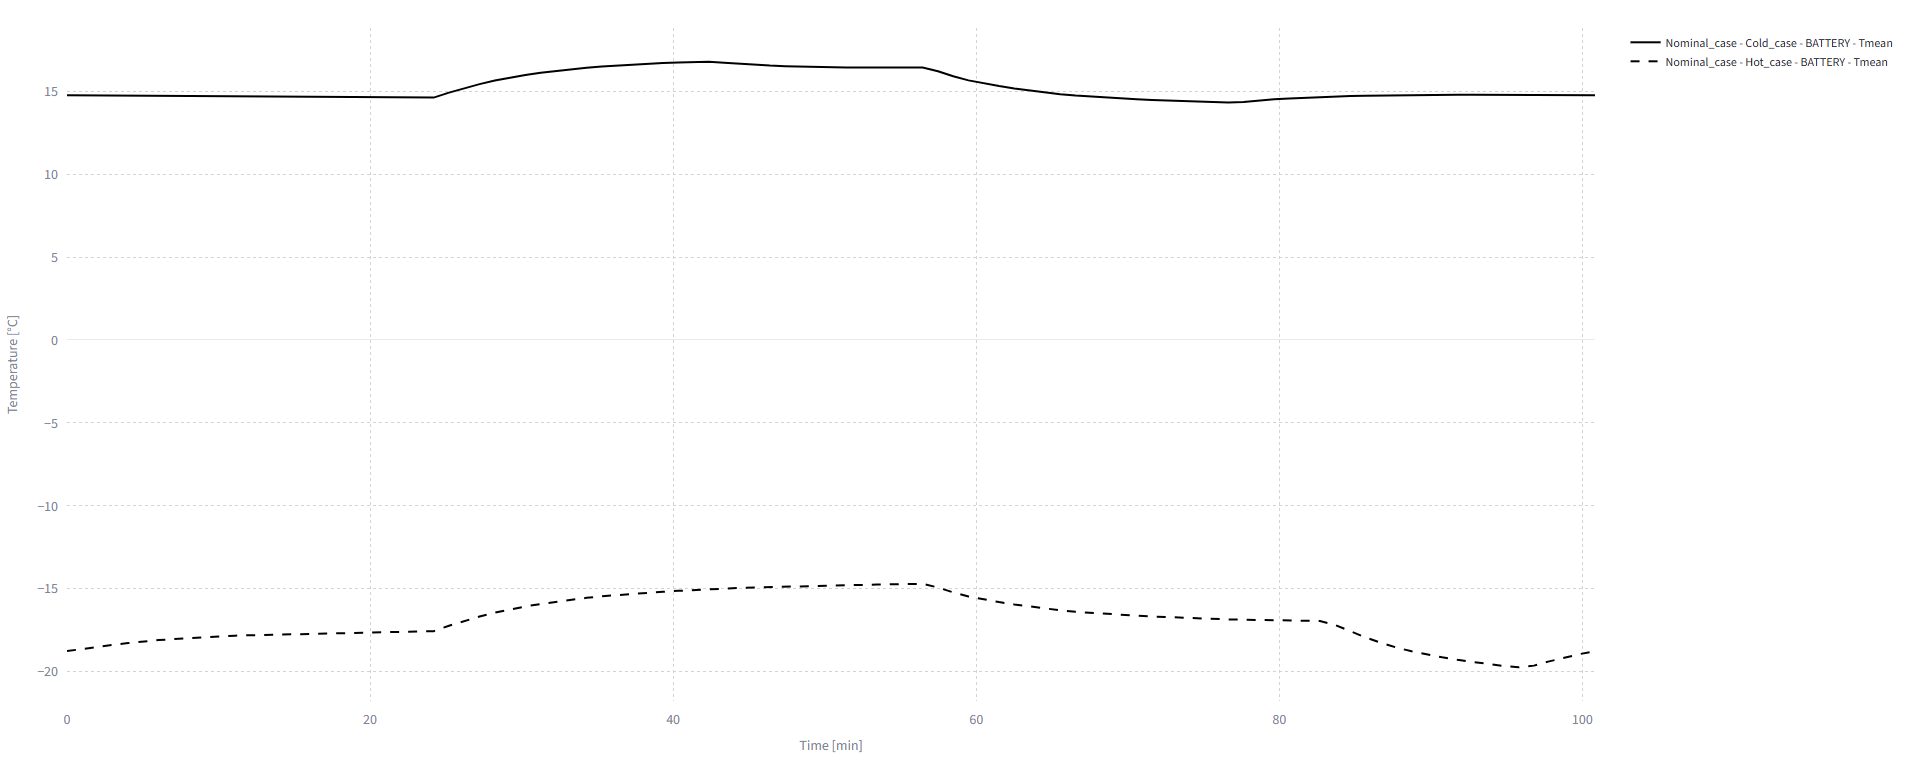
\includegraphics[
        width=1.0\textwidth,
        keepaspectratio
    ]{Figures/09/battery_temperature_difference.png}
    \caption{Nominal-minus-hot and nominal-minus-cold differences in mean
    battery temperature.}
    \label{fig:battery_temperature_difference}
\end{figure}

Table~\ref{tab:case_difference_snapshot} extends the same representation to
several groups and results at $95.80\,\mathrm{min}$. At this instant, the
nominal battery is $19.75\,^{\circ}\mathrm{C}$ colder than the hot battery
and $14.79\,^{\circ}\mathrm{C}$ warmer than the cold battery. The large
$42.96\,^{\circ}\mathrm{C}$ nominal-minus-hot difference in
\texttt{SOLAR\_PANEL\_1} occurs because the nominal panel is illuminated while
the hot case is still in eclipse. The table also separates this orbital-phase
effect from the prescribed internal dissipations: the battery load difference
is $-12.25\,\mathrm{W}$ for nominal minus hot and $1.13\,\mathrm{W}$ for
nominal minus cold.

% File: Tables/table_case_difference_snapshot.tex
% Usage: \CaseDifferenceSnapshotTable[0.98\textwidth]
% The values correspond to the selected output instant t = 95.80 min.

\newcommand{\CaseDifferenceSnapshotTable}[1][0.98\textwidth]{%
\begin{table}[H]
    \centering
    \caption{Case differences at \(t=95.80\) min, corresponding to the
    maximum absolute nominal--hot difference in mean battery temperature.}
    \label{tab:case_difference_snapshot}
    \footnotesize
    \renewcommand{\arraystretch}{1.18}
    \setlength{\tabcolsep}{3.4pt}
    \resizebox{#1}{!}{%
    \begin{tabular}{|l|c|c|c|c|c|c|}
        \hline
        & \multicolumn{3}{c|}{\textbf{Nominal -- Hot}} &
          \multicolumn{3}{c|}{\textbf{Nominal -- Cold}} \\ \cline{2-7}
        \textbf{Group} &
        \textbf{$\Delta T_{\mathrm{mean}}$ [$^\circ$C]} &
        \textbf{$\Delta Q_S$ [W]} &
        \textbf{$\Delta Q_I$ [W]} &
        \textbf{$\Delta T_{\mathrm{mean}}$ [$^\circ$C]} &
        \textbf{$\Delta Q_S$ [W]} &
        \textbf{$\Delta Q_I$ [W]} \\ \hline
        \texttt{SOLAR\_PANEL\_1} & 42.96  & 372.87 & 0.00   & 25.57 & 15.07  & 0.00  \\ \hline
        \texttt{OBC\_BOX}        & -16.33 & 4.54   & -1.00  & 12.89 & 0.18   & 2.00  \\ \hline
        \texttt{RADIATOR}         & -11.98 & 12.65  & 0.00   & 9.54  & 0.51   & 0.00  \\ \hline
        \texttt{BATTERY}          & -19.75 & 0.002  & -12.25 & 14.79 & $<0.001$ & 1.13 \\ \hline
    \end{tabular}%
    }
    \par\vspace{0.3em}
    \begin{minipage}{#1}
        \footnotesize
        \textit{Note:} Differences follow the reference-minus-comparison
        convention defined in Equation~\eqref{eq:results_case_difference}.
    \end{minipage}
\end{table}%
}

\CaseDifferenceSnapshotTable[0.8\textwidth]


\subsection{Temperature Variations and Interface Differences}
\label{subsec:temperature_interface_comparison}

The temperature-change envelopes of \texttt{BODY\_PANEL} over a nominal
$30\,\mathrm{min}$ interval are represented in
Figure~\ref{fig:body_panel_deltaT_comparison}. The effective interval obtained
from the output-time vector is $30.25\,\mathrm{min}$. Negative values identify
cooling over the selected window and positive values identify heating.

\begin{figure}[H]
    \centering
    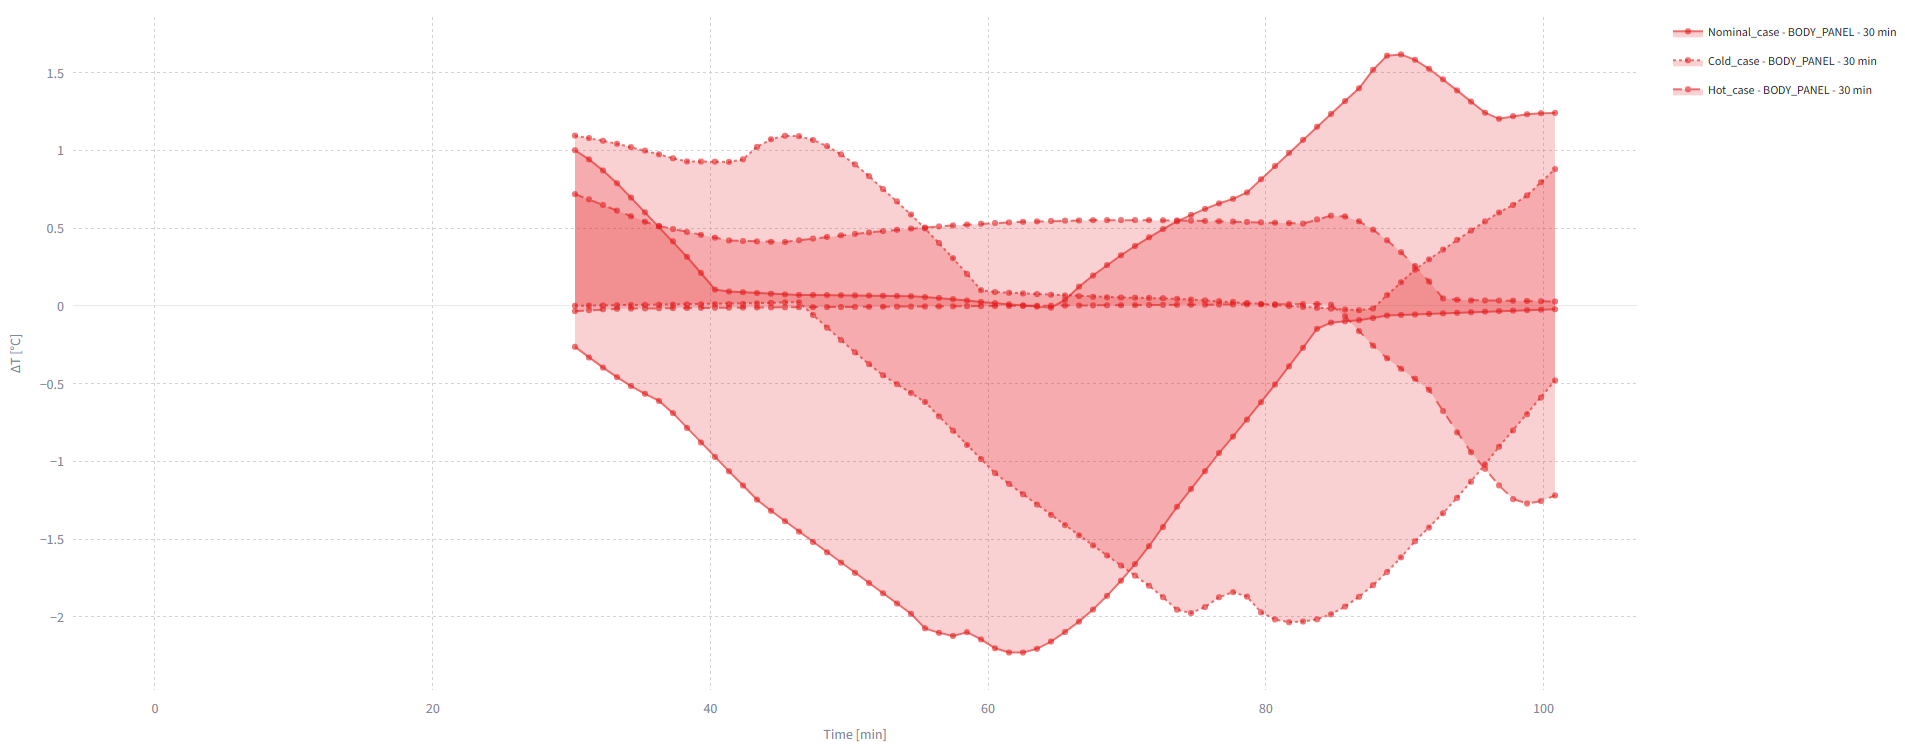
\includegraphics[
        width=0.9\textwidth,
        keepaspectratio
    ]{Figures/09/body_panel_deltaT_comparison.png}
    \caption{Temperature-change envelopes of \texttt{BODY\_PANEL} over a
    $30\,\mathrm{min}$ window.}
    \label{fig:body_panel_deltaT_comparison}
\end{figure}

The largest absolute variation occurs in the nominal case, with a decrease of
$2.23\,^{\circ}\mathrm{C}$ at $62.52\,\mathrm{min}$. The cold case reaches
$2.03\,^{\circ}\mathrm{C}$ at $81.68\,\mathrm{min}$, while the hot case
remains below $1.28\,^{\circ}\mathrm{C}$. The highest absolute temperature
case is therefore not the one with the fastest change over this interval. The
nominal and cold envelopes widen after their respective eclipse transitions,
whereas the shorter hot eclipse limits the magnitude of the delayed cooling
and reheating response.

The connected-node differences between \texttt{OBC\_BOX} and
\texttt{RADIATOR} are shown in
Figure~\ref{fig:obc_radiator_interface_comparison}. At each instant, the upper
and lower curves correspond to the connected pair that produces the largest
absolute difference for that case. The pair can change during the simulation,
so the figure is interpreted together with the maximum-value summary in
Table~\ref{tab:multicase_interface_summary}.

\begin{figure}[H]
    \centering
    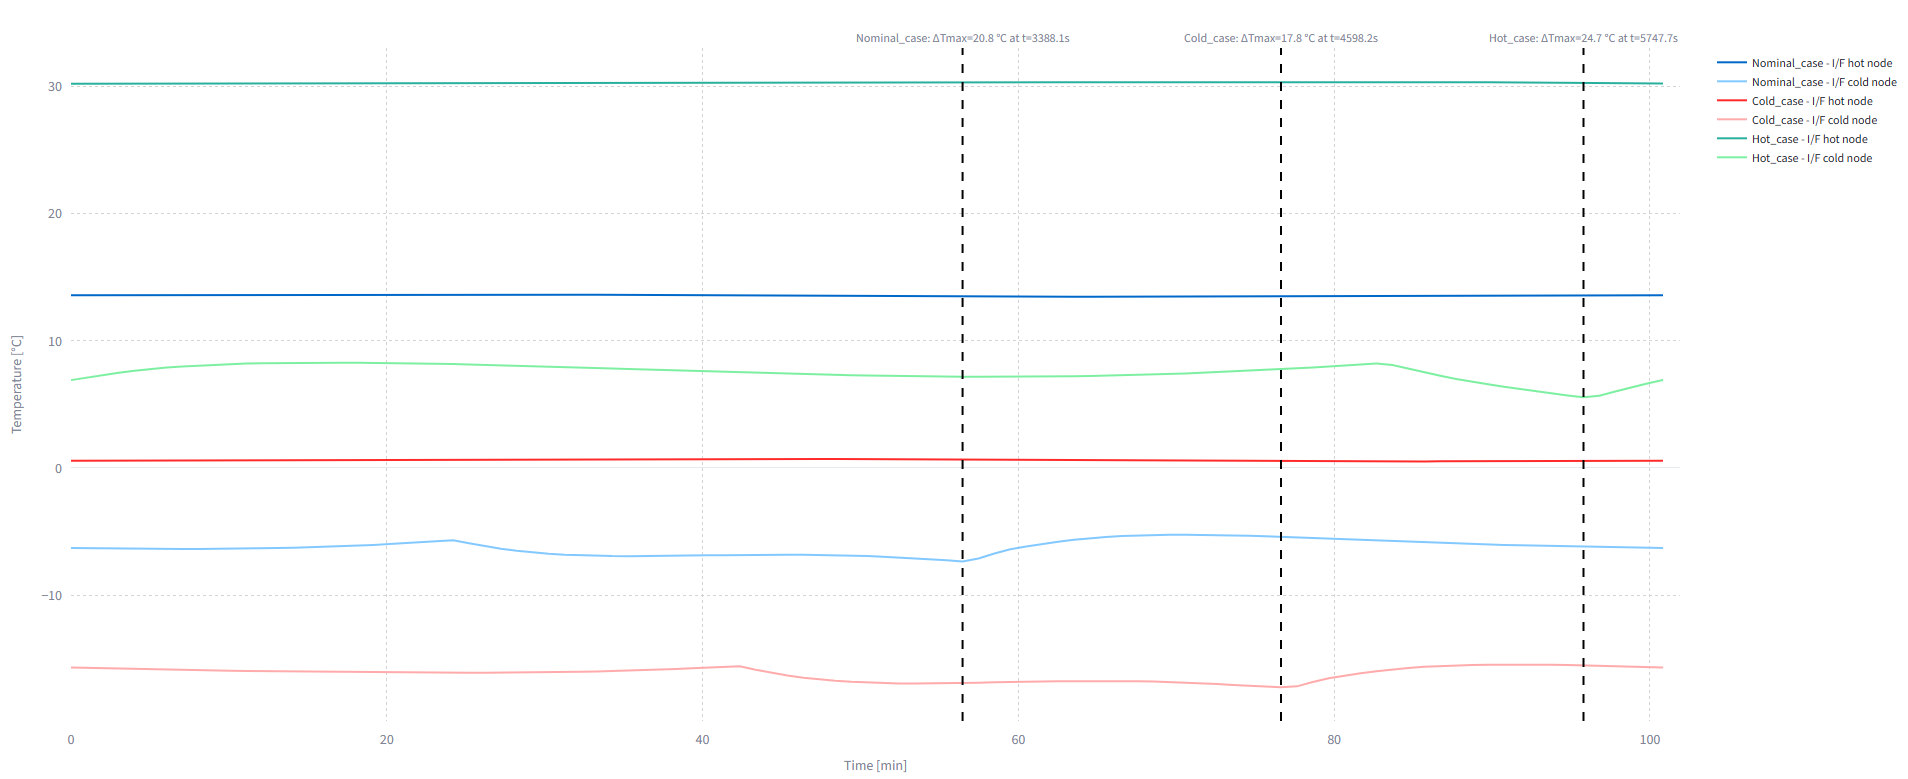
\includegraphics[
        width=0.8\textwidth,
        keepaspectratio
    ]{Figures/09/obc_radiator_interface_comparison.png}
    \caption{Critical connected-node temperatures between
    \texttt{OBC\_BOX} and \texttt{RADIATOR}.}
    \label{fig:obc_radiator_interface_comparison}
\end{figure}

% File: Tables/table_multicase_interface_summary.tex
% Usage: \MultiCaseInterfaceSummaryTable[0.98\textwidth]
% Values obtained from the OBC_BOX--RADIATOR interface exports.

\newcommand{\MultiCaseInterfaceSummaryTable}[1][0.98\textwidth]{%
\begin{table}[H]
    \centering
    \caption{Maximum connected-node temperature difference between
    \texttt{OBC\_BOX} and \texttt{RADIATOR} in the three transient cases.}
    \label{tab:multicase_interface_summary}
    \footnotesize
    \renewcommand{\arraystretch}{1.18}
    \setlength{\tabcolsep}{3.6pt}
    \resizebox{#1}{!}{%
    \begin{tabular}{|l|c|c|c|c|c|c|}
        \hline
        \textbf{Case} &
        \textbf{$|\Delta T|_{\max}$ [$^\circ$C]} &
        \textbf{Time [min]} &
        \textbf{$T_{\mathrm{hot}}$ [$^\circ$C]} &
        \textbf{$T_{\mathrm{cold}}$ [$^\circ$C]} &
        \textbf{Hot--cold nodes} &
        \textbf{Coupling} \\ \hline
        Nominal & 20.81 & 56.47 & 13.44 & -7.37  & 31023--35506 & GR \\ \hline
        Hot     & 24.67 & 95.80 & 30.22 & 5.56   & 31023--35506 & GR \\ \hline
        Cold    & 17.78 & 76.64 & 0.52  & -17.25 & 31017--35502 & GR \\ \hline
    \end{tabular}%
    }
\end{table}%
}

\MultiCaseInterfaceSummaryTable[0.98\textwidth]

The maximum interface difference increases from
$17.78\,^{\circ}\mathrm{C}$ in the cold case to
$20.81\,^{\circ}\mathrm{C}$ in the nominal case and
$24.67\,^{\circ}\mathrm{C}$ in the hot case. The nominal and hot maxima are
formed by nodes 31023 and 35506, while the cold maximum involves nodes 31017
and 35502. Both conductive and radiative couplings are present in every
critical pair. The hot environment therefore not only shifts both components
to higher temperatures, but also produces the largest separation between the
selected OBC and radiator nodes.


\subsection{Heat Flows and Net Energy Transfer}
\label{subsec:heat_flow_energy_comparison}

The total heat flow for the source--target selection \texttt{BATTERY}--
\texttt{BODY\_PLATE\_INF} follows the convention established in
Section~\ref{sec:heat_flow_evolution}. Positive values indicate heat entering
the battery from the plate, whereas negative values indicate heat leaving the
battery. Figure~\ref{fig:battery_body_plate_heat_flow_comparison} compares
$Q_{\mathrm{GT}}$ for the three cases.

\begin{figure}[H]
    \centering
    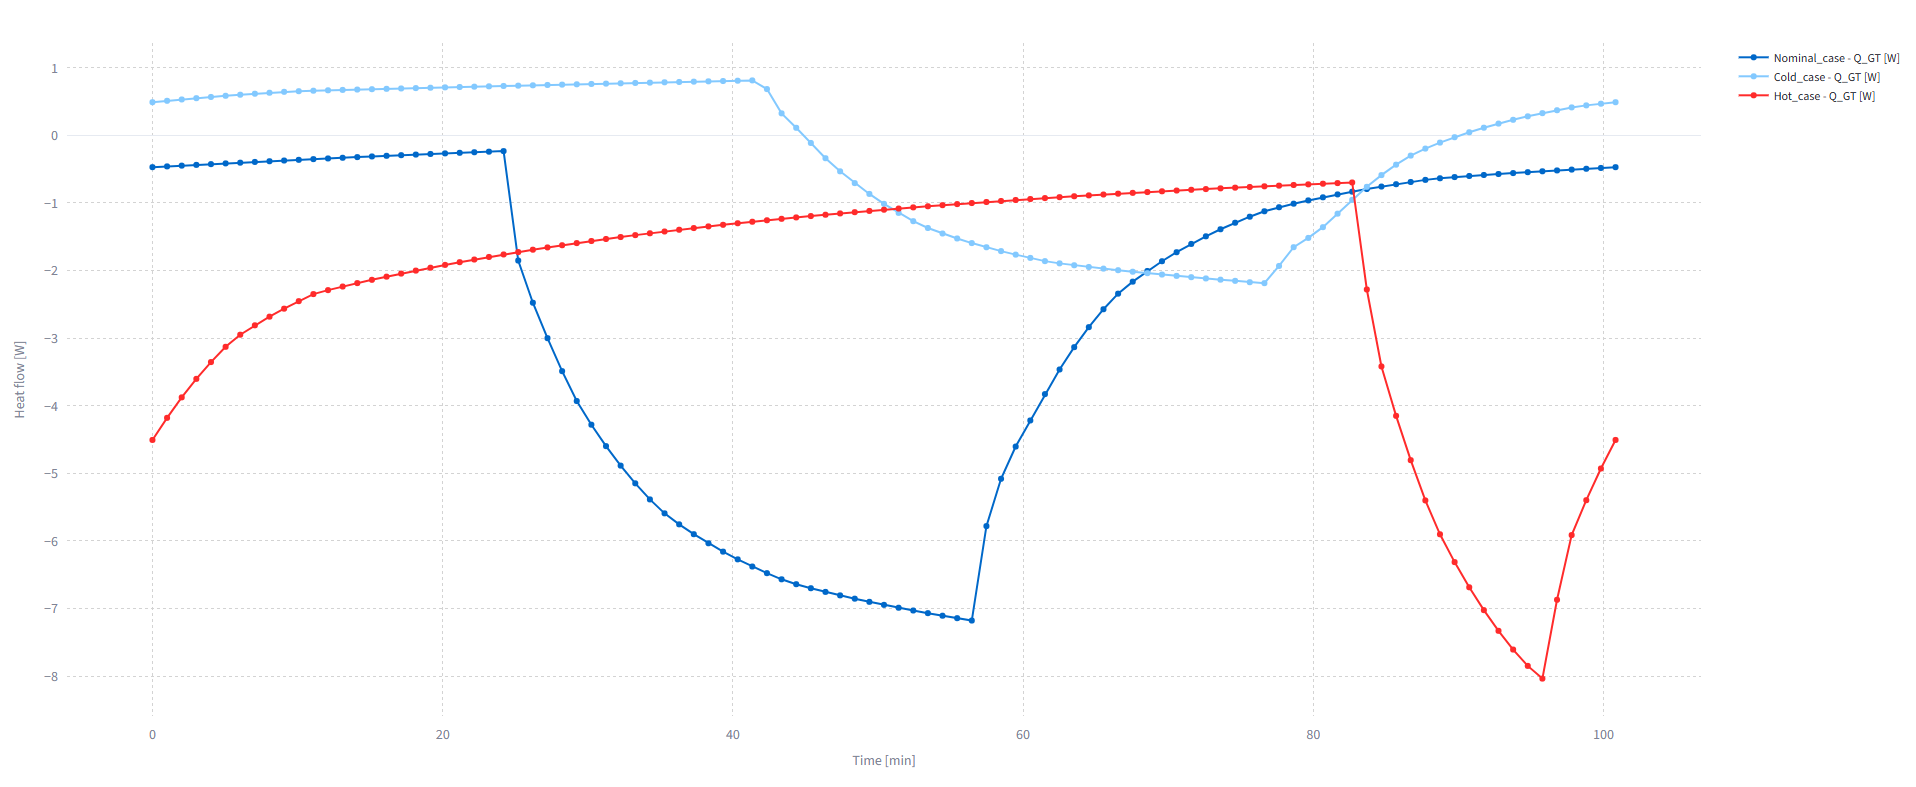
\includegraphics[
        width=0.9\textwidth,
        keepaspectratio
    ]{Figures/09/battery_body_plate_total_heat_flow_comparison.png}
    \caption{Total heat flow between \texttt{BATTERY} and
    \texttt{BODY\_PLATE\_INF}. Negative values indicate heat leaving the
    battery.}
    \label{fig:battery_body_plate_heat_flow_comparison}
\end{figure}

The nominal and hot flows remain negative throughout the interval. Their most
negative values are $-7.18\,\mathrm{W}$ and $-8.04\,\mathrm{W}$,
respectively, showing that the hotter battery continuously rejects heat to its
supporting plate. The cold case ranges from $0.81\,\mathrm{W}$ to
$-2.19\,\mathrm{W}$ and changes direction. During part of the orbit the plate
warms the battery, while the sign reverses when the battery becomes the warmer
side of the connection. In all three cases, the conductive contribution is
dominant and the radiative term only modifies the total magnitude.

The corresponding \textit{Case difference} curves are represented in
Figure~\ref{fig:battery_body_plate_heat_flow_difference}. Nominal minus hot
ranges from $-6.17$ to $7.50\,\mathrm{W}$, while nominal minus cold ranges
from $-7.19$ to $1.06\,\mathrm{W}$. The sign changes show that a single
constant offset cannot describe the effect of the environmental cases. The
relative heat transfer depends on the different eclipse intervals and on the
case-dependent battery dissipation.

\begin{figure}[H]
    \centering
    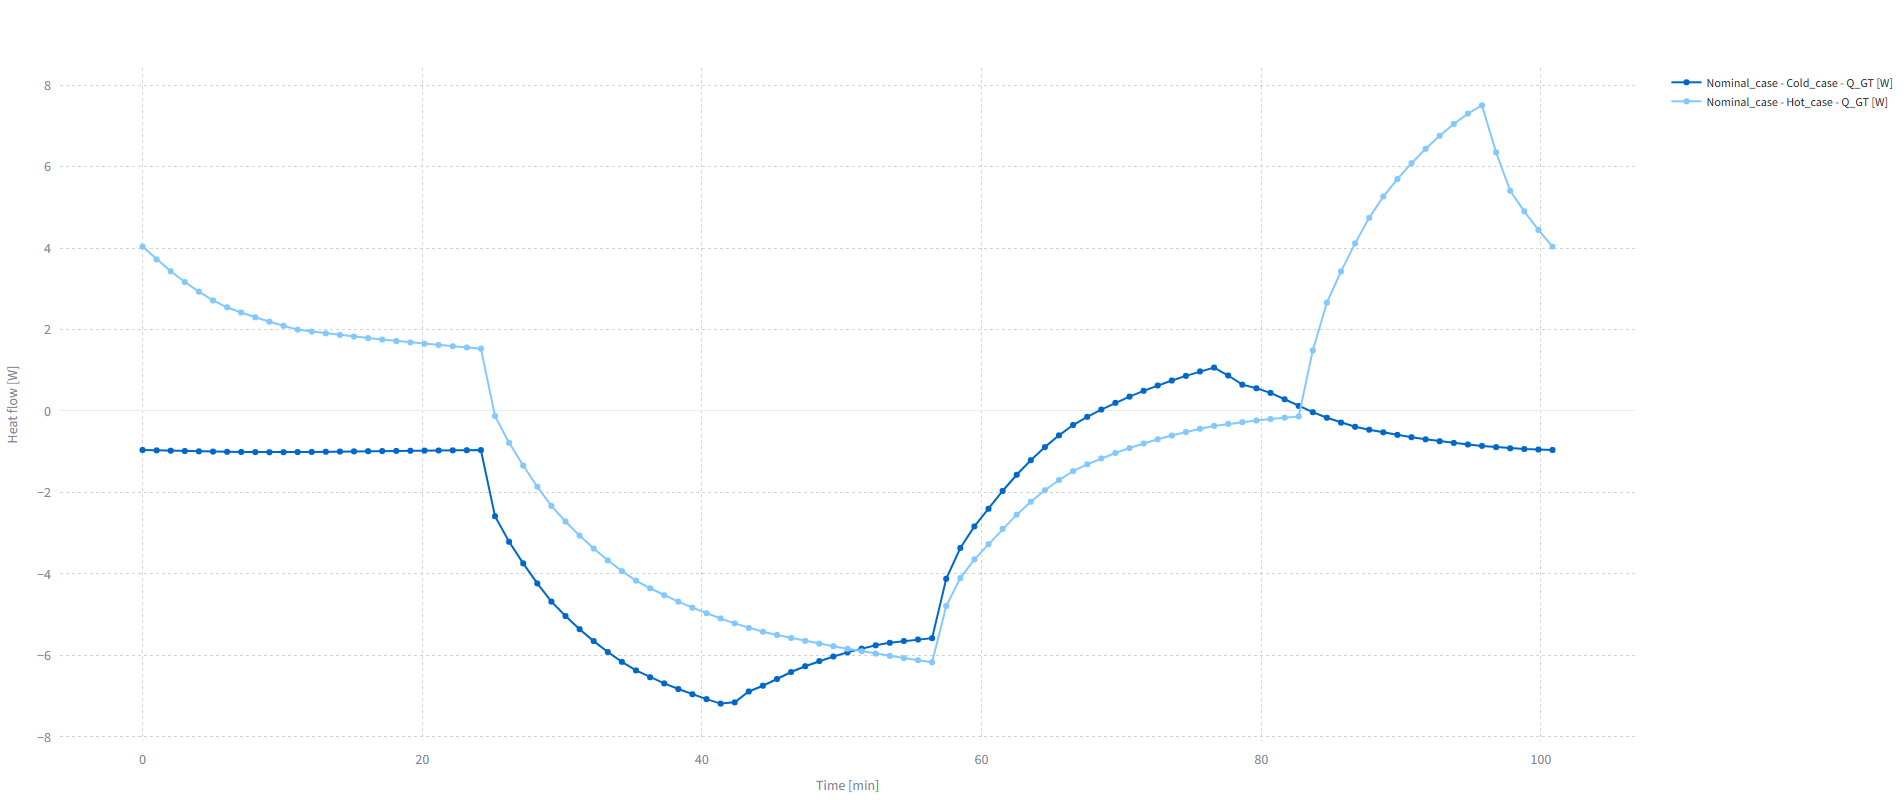
\includegraphics[
        width=0.9\textwidth,
        keepaspectratio
    ]{Figures/09/battery_body_plate_heat_flow_difference.png}
    \caption{Nominal-minus-hot and nominal-minus-cold differences in total
    battery-to-plate heat flow.}
    \label{fig:battery_body_plate_heat_flow_difference}
\end{figure}

The complete battery thermal balance and its time integral are compared in
Figure~\ref{fig:battery_net_energy_comparison}. The integral starts from zero
for each case and represents the net thermal-energy change relative to the
initial instant. It can increase or decrease according to the sign of
$Q_{\mathrm{balance}}$ and must not be interpreted as the absolute energy
stored in the battery.

\begin{figure}[H]
    \centering
    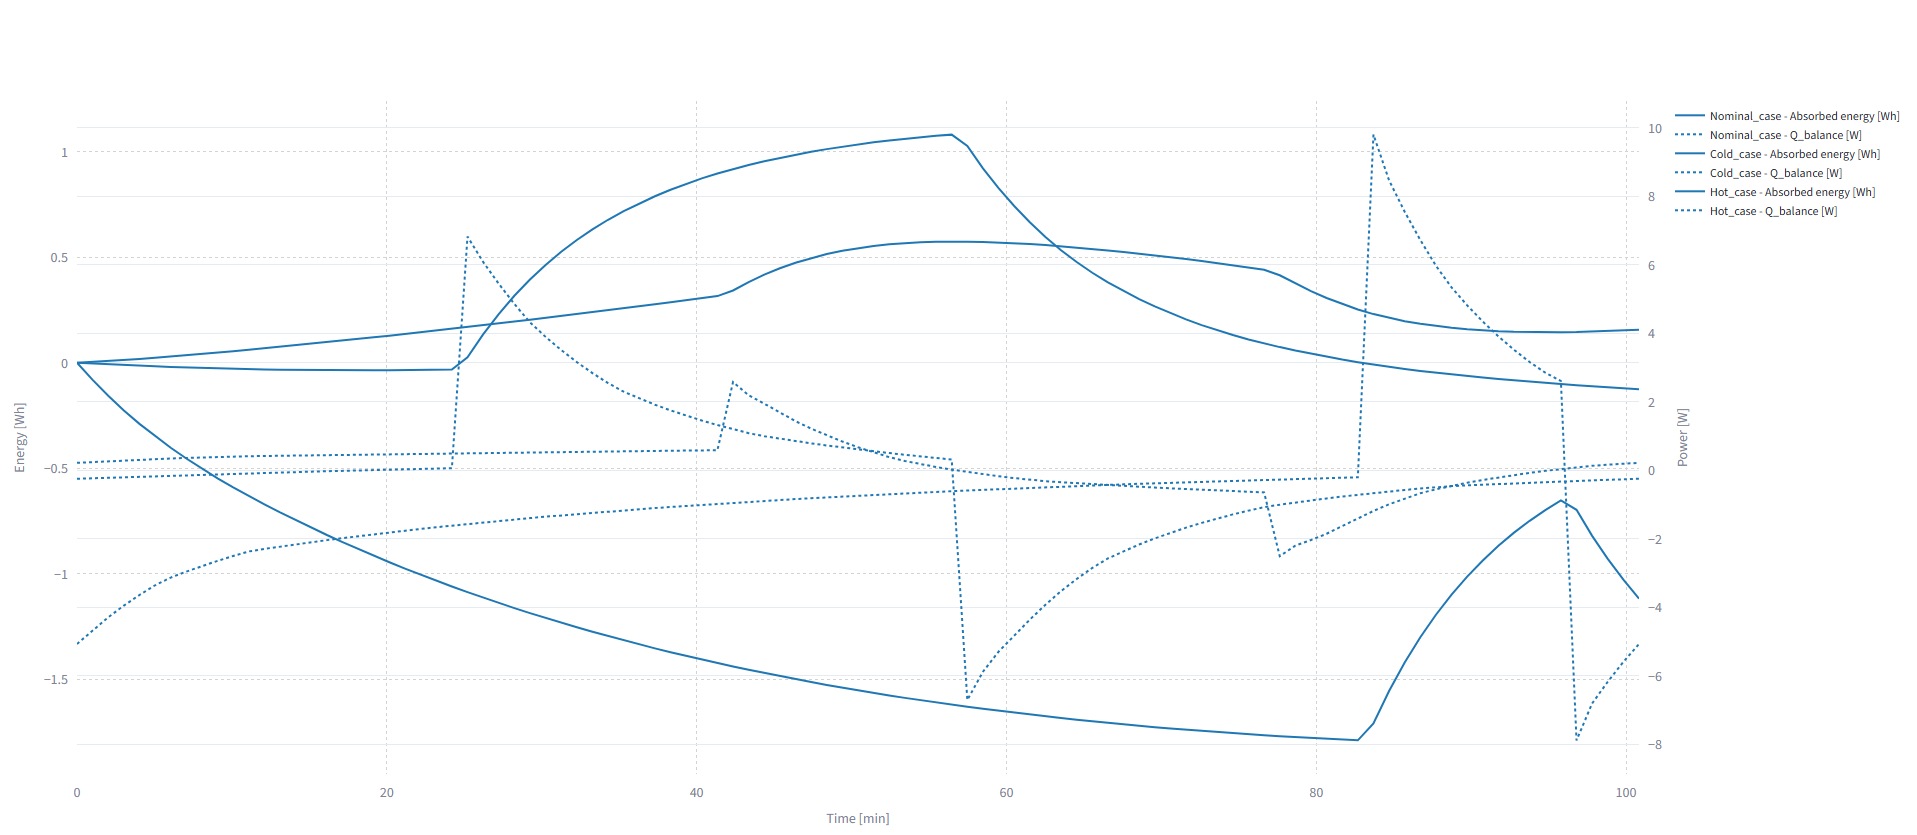
\includegraphics[
        width=0.9\textwidth,
        keepaspectratio
    ]{Figures/09/battery_net_thermal_energy_comparison.png}
    \caption{Battery thermal balance and net thermal-energy change relative to
    the initial instant.}
    \label{fig:battery_net_energy_comparison}
\end{figure}

The nominal curve initially rises to $1.08\,\mathrm{Wh}$ and subsequently
falls to $-0.13\,\mathrm{Wh}$ at the end of the simulation. The cold case
reaches $0.57\,\mathrm{Wh}$ and ends at $0.16\,\mathrm{Wh}$, indicating a
small positive net change over the analysed interval. The hot case presents a
predominantly negative integral, reaches $-1.79\,\mathrm{Wh}$ before its late
eclipse transition and finishes at $-1.12\,\mathrm{Wh}$. These values describe
the balance of all selected thermal contributions and are independent of the
electrical energy stored by the battery model.

Figure~\ref{fig:battery_thermal_balance_energy_difference} provides an
additional \textit{Case difference} example for nominal minus cold. The power
difference ranges from approximately $-6.65$ to $6.32\,\mathrm{W}$, while the
difference between their integrated thermal-energy changes remains between
$-0.35$ and $0.58\,\mathrm{Wh}$ and ends at $-0.28\,\mathrm{Wh}$. The energy
difference follows the accumulated effect of the signed power difference and
therefore varies more gradually than the instantaneous curve.

\begin{figure}[H]
    \centering
    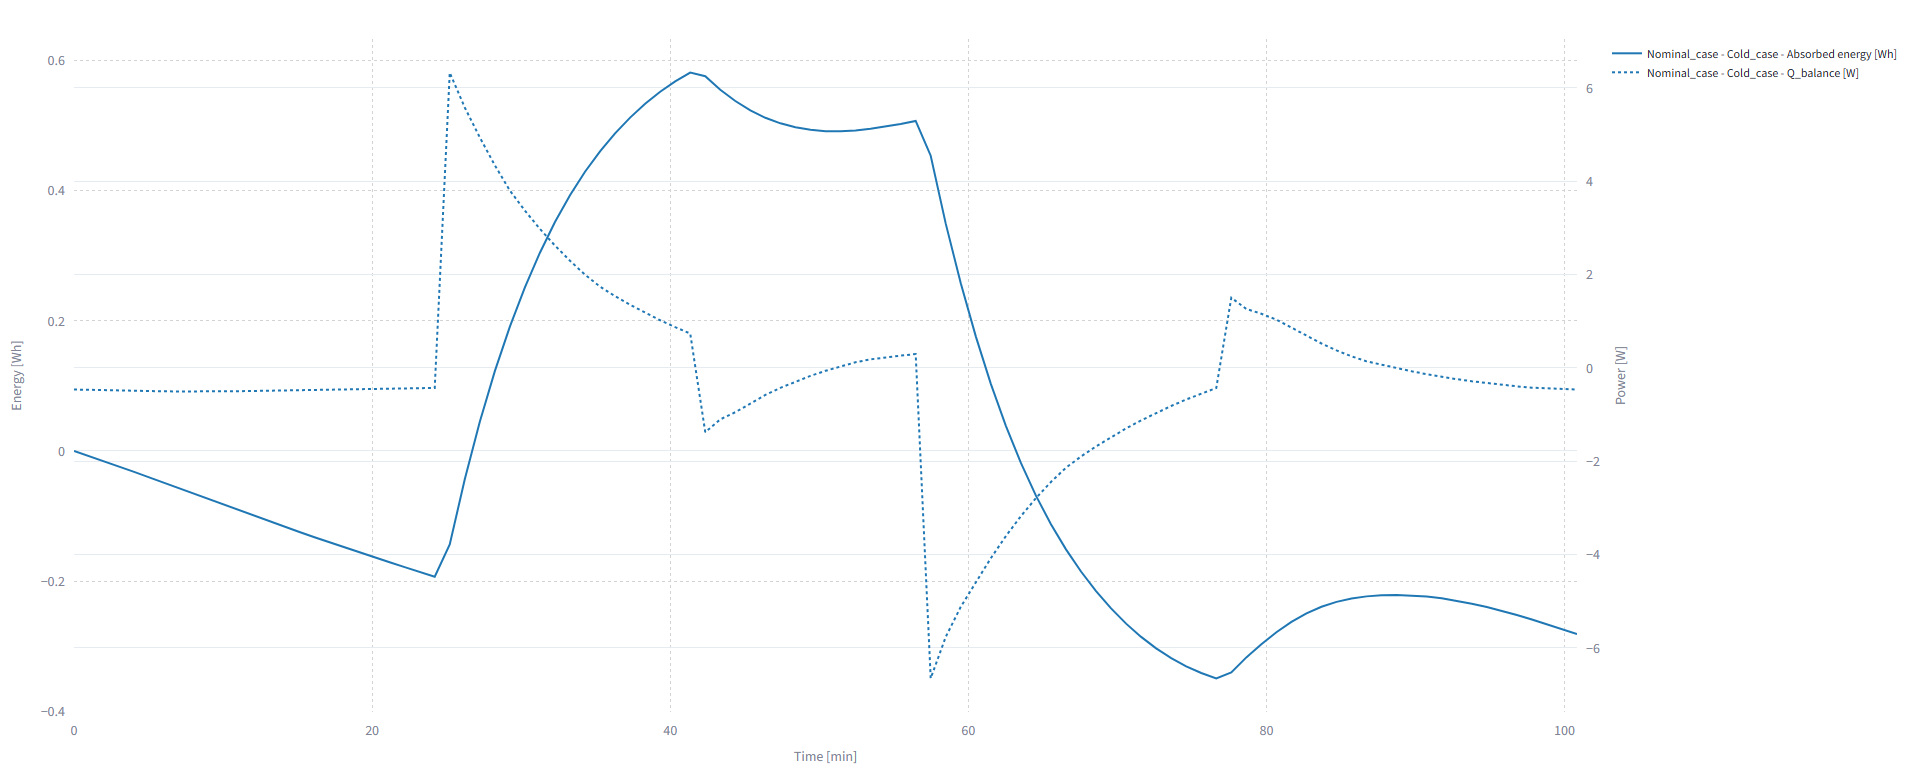
\includegraphics[
        width=0.98\textwidth,
        keepaspectratio
    ]{Figures/09/battery_thermal_balance_energy_difference.png}
    \caption{Nominal-minus-cold difference in battery thermal balance and net
    thermal-energy change.}
    \label{fig:battery_thermal_balance_energy_difference}
\end{figure}


\section{Electrical and Battery Response}
\label{sec:electrical_battery_comparison}

The same solar group, load groups, thermo-optical definition, efficiency
expression and battery parameters are used for all three cases. The electrical
comparison therefore reflects the case-dependent absorbed solar load, panel
temperature, internal dissipations and battery temperature.


\subsection{Solar Generation and Load Demand}
\label{subsec:solar_load_comparison}

Figure~\ref{fig:solar_electrical_balance_comparison} compares the estimated
solar electrical generation $Q_{S,\mathrm{elec}}$ with the demand formed by
the selected equipment groups. Generation becomes zero during the eclipse of
each case, while the load changes according to the dissipations defined in
Table~\ref{tab:internal_heat_loads}. The hot case therefore combines the
largest load with the shortest generation interruption; the cold case combines
the smallest load with the longest eclipse.

\begin{figure}[H]
    \centering
    
\includegraphics[
        width=0.9\textwidth,
        keepaspectratio
    ]{Figures/09/solar_electrical_balance_comparison.png}
    \caption{Estimated solar electrical generation and selected load demand
    in the three cases.}
    \label{fig:solar_electrical_balance_comparison}
\end{figure}

The maximum instantaneous electrical generation is
$326.25\,\mathrm{W}$ in the nominal case, $316.03\,\mathrm{W}$ in the hot
case and $317.53\,\mathrm{W}$ in the cold case. The hot case receives the
largest absorbed solar load, but its higher panel temperature reduces the
conversion efficiency and prevents it from producing the largest instantaneous
value. The total generated energy is nevertheless highest in the hot case
because of its much longer illuminated interval.

The difference curves in
Figure~\ref{fig:solar_electrical_generation_difference} are dominated by the
non-coincident eclipse intervals. Nominal minus hot falls to approximately
$-289\,\mathrm{W}$ when the nominal case enters eclipse while the hot case
remains illuminated, and later rises to about $285\,\mathrm{W}$ when the hot
case enters its late eclipse. Nominal minus cold reaches
$326\,\mathrm{W}$ after nominal illumination resumes while the cold case
remains in eclipse. When both cases share the same illumination state, the
remaining separation is associated with the different incident loads and
panel-temperature-dependent efficiencies.

\begin{figure}[H]
    \centering
    
\includegraphics[
        width=0.9\textwidth,
        keepaspectratio
    ]{Figures/09/solar_electrical_generation_difference.png}
    \caption{Nominal-minus-hot and nominal-minus-cold differences in estimated
    solar electrical generation.}
    \label{fig:solar_electrical_generation_difference}
\end{figure}

The integrated results are collected in
Table~\ref{tab:multicase_electrical_summary}. The hot case generates
$421.60\,\mathrm{Wh}$ and demands $33.75\,\mathrm{Wh}$, whereas the nominal
case generates $328.07\,\mathrm{Wh}$ and demands $25.58\,\mathrm{Wh}$. The
cold case has the lowest generation, $306.41\,\mathrm{Wh}$, but its reduced
internal loads limit the demand to $6.92\,\mathrm{Wh}$. All three direct net
balances remain positive over the complete interval. The direct deficits are
restricted to eclipse and equal $11.29\,\mathrm{Wh}$, $6.61\,\mathrm{Wh}$
and $3.24\,\mathrm{Wh}$ for the nominal, hot and cold cases, respectively.
These values are evaluated before the battery restrictions are applied.

% File: Tables/table_multicase_electrical_summary.tex
% Usage: \MultiCaseElectricalSummaryTable[0.94\textwidth]
% Energies are obtained by trapezoidal integration of the exported power
% profiles over the complete simulated interval.

\newcommand{\MultiCaseElectricalSummaryTable}[1][0.94\textwidth]{%
\begin{table}[H]
    \centering
    \caption{Integrated solar generation and selected load demand for the
    nominal, hot and cold transient cases.}
    \label{tab:multicase_electrical_summary}
    \footnotesize
    \renewcommand{\arraystretch}{1.18}
    \setlength{\tabcolsep}{4.2pt}
    \resizebox{#1}{!}{%
    \begin{tabular}{|l|c|c|c|c|c|}
        \hline
        \textbf{Case} &
        \textbf{Generated energy [Wh]} &
        \textbf{Load energy [Wh]} &
        \textbf{Direct surplus [Wh]} &
        \textbf{Direct deficit [Wh]} &
        \textbf{Net balance [Wh]} \\ \hline
        Nominal & 328.07 & 25.58 & 313.78 & 11.29 & 302.49 \\ \hline
        Hot     & 421.60 & 33.75 & 394.46 & 6.61  & 387.85 \\ \hline
        Cold    & 306.41 & 6.92  & 302.73 & 3.24  & 299.49 \\ \hline
    \end{tabular}%
    }
    \par\vspace{0.3em}
    \begin{minipage}{#1}
        \footnotesize
        \textit{Note:} Direct surplus and deficit are the time integrals of
        the positive and negative parts, respectively, of
        \(Q_{S,\mathrm{elec}}-Q_{\mathrm{load}}\), before applying the battery
        operating limits.
    \end{minipage}
\end{table}%
}

\MultiCaseElectricalSummaryTable[0.85\textwidth]


\subsection{Battery State and Operating Limits}
\label{subsec:battery_comparison}

Battery operation is calculated independently for each physical case. Direct
subtraction is not used for SOC, voltage or current because the difference
between two battery states does not describe an independent operating state.
The absolute SOC curves in Figure~\ref{fig:battery_soc_comparison} provide the
main comparison.

\begin{figure}[H]
    \centering
    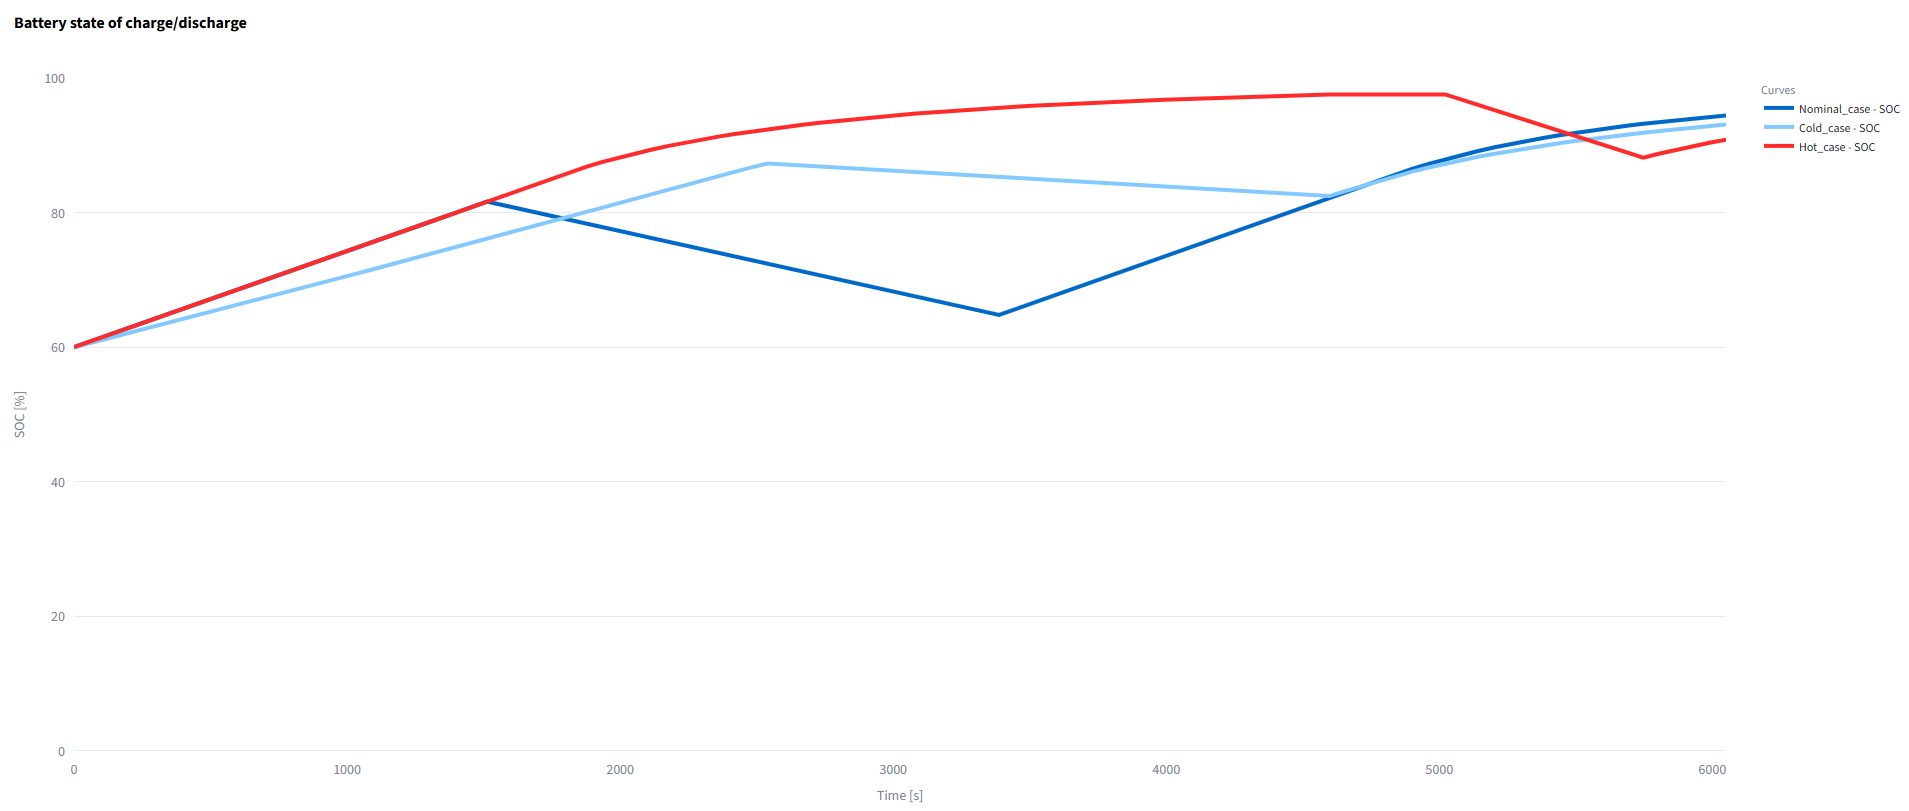
\includegraphics[
        width=0.82\textwidth,
        keepaspectratio
    ]{Figures/09/battery_soc_comparison.png}
    \caption{Battery state of charge obtained with the common battery
    configuration.}
    \label{fig:battery_soc_comparison}
\end{figure}

All cases begin at $60\%$ SOC. The nominal battery charges before eclipse,
discharges while solar generation is absent and subsequently recovers to a
final value of $94.43\%$. The cold battery follows the same sequence with a
longer discharge interval but a substantially lower demand, ending at
$93.08\%$. The hot battery reaches the largest maximum SOC,
$97.56\%$, before its late eclipse. Its higher eclipse load then causes the
strongest discharge and the remaining illuminated interval only restores the
SOC to $90.84\%$. Final SOC therefore depends on the timing of generation and
demand as well as on their total integrated values.

The battery temperatures and thermal charging restrictions are compared in
Figure~\ref{fig:battery_temperature_derating_comparison}. Charge and discharge
efficiencies remain fixed at $0.98$ in all cases. The nominal and hot battery
temperatures remain inside the unrestricted charging interval, so their
charge-derating factors stay equal to one. The cold battery remains between
$3.66$ and $4.46\,^{\circ}\mathrm{C}$, inside the lower $5\,^{\circ}\mathrm{C}$
derating ramp. Its factor varies from $0.733$ to $0.892$ and restricts charging
throughout the complete $100.84\,\mathrm{min}$ simulation.

\begin{figure}[H]
    \centering
    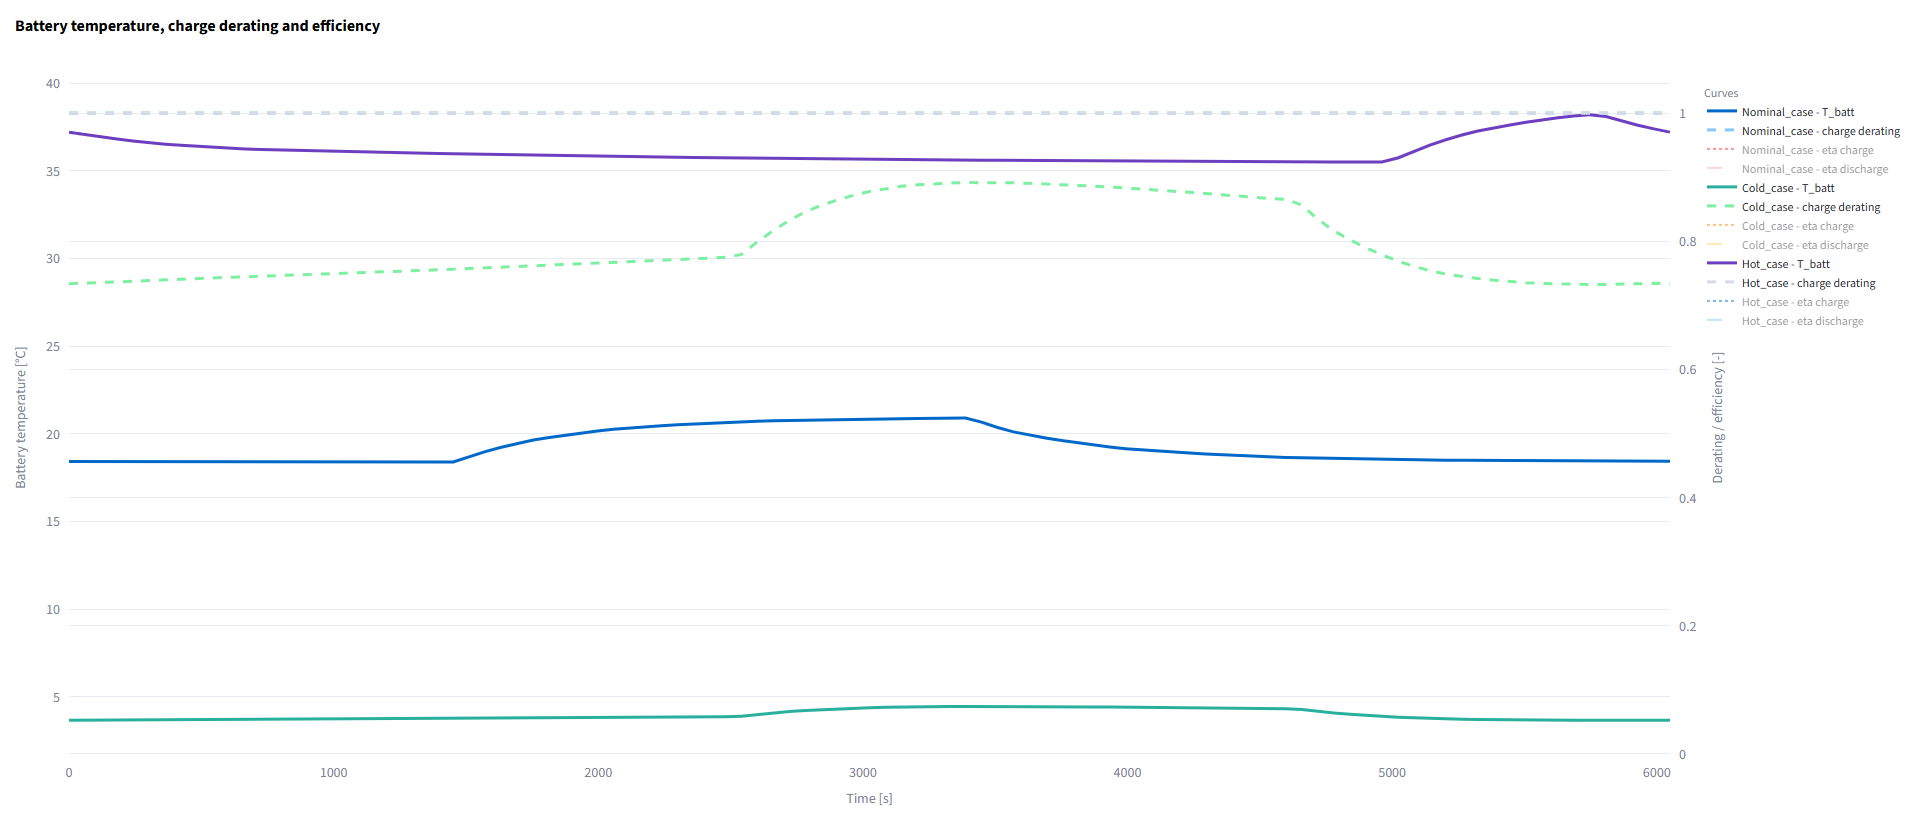
\includegraphics[
        width=0.85\textwidth,
        keepaspectratio
    ]{Figures/09/battery_temperature_derating_comparison.png}
    \caption{Battery temperature, charge-derating factor and electrical
    efficiencies in the three cases.}
    \label{fig:battery_temperature_derating_comparison}
\end{figure}

The lower accepted charge current limits the cold-case maximum charge power to
$30.24\,\mathrm{W}$, compared with approximately $35.4\,\mathrm{W}$ in the
nominal and hot cases. Despite this restriction, the available generation and
stored energy remain sufficient to supply the complete selected load. The
unserved-load energy is negligible in every simulation.

Terminal voltage and charge/discharge currents are shown separately in
Figure~\ref{fig:battery_voltage_current_comparison} to avoid overlapping nine
curves in a single graph. The same battery parameters and axis definitions are
retained in the three subfigures.

\begin{figure}[H]
    \centering

    \begin{subfigure}[t]{0.85\textwidth}
        \centering
        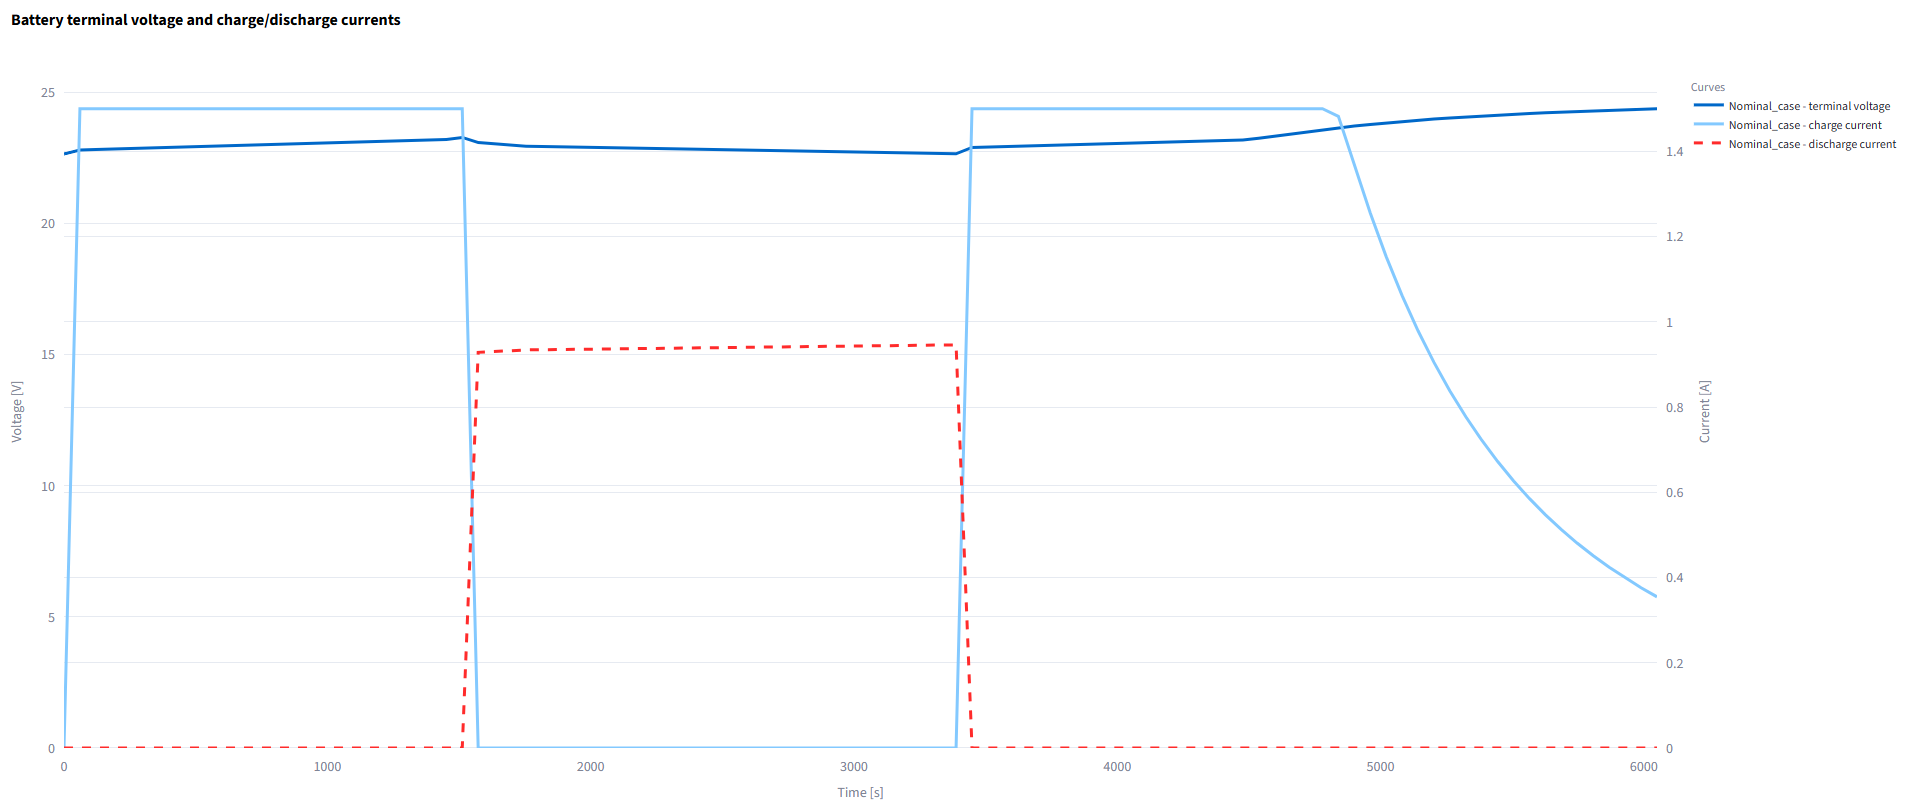
\includegraphics[
            width=\textwidth,
            keepaspectratio
        ]{Figures/09/nominal_battery_voltage_current.png}
        \caption{Nominal case.}
        \label{fig:nominal_battery_voltage_current_ch9}
    \end{subfigure}
\end{figure}

\begin{figure}[H]
    \ContinuedFloat
    \centering

    \begin{subfigure}[t]{0.8\textwidth}
        \centering
        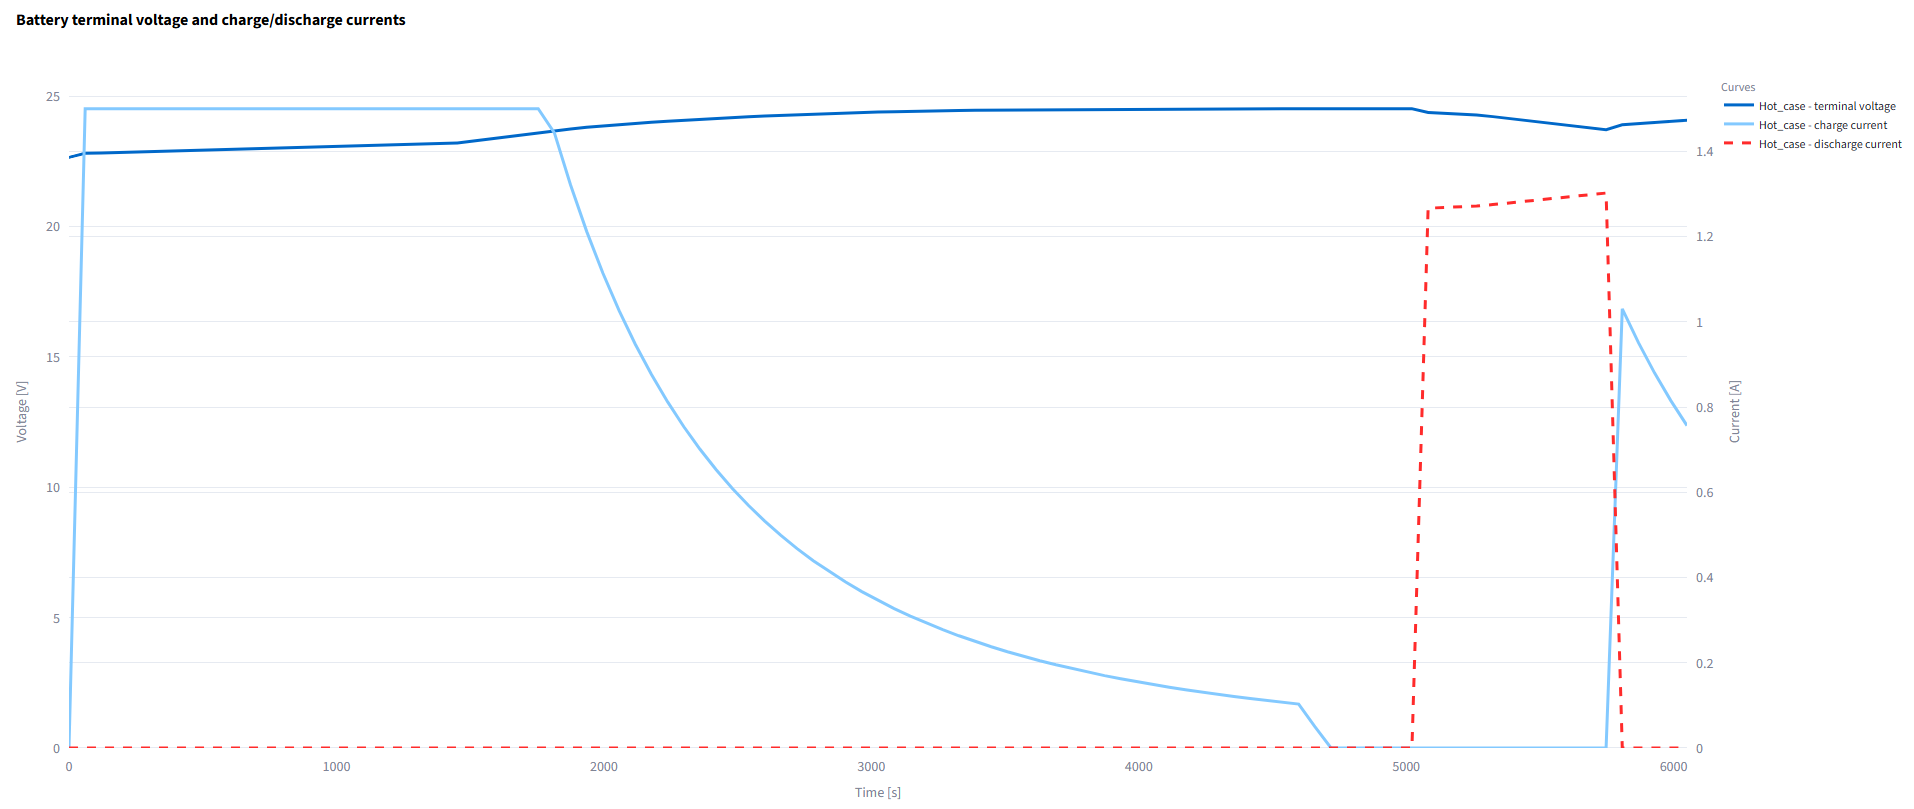
\includegraphics[
            width=\textwidth,
            keepaspectratio
        ]{Figures/09/hot_battery_voltage_current.png}
        \caption{Hot case.}
        \label{fig:hot_battery_voltage_current_ch9}
    \end{subfigure}

\end{figure}

\begin{figure}[H]
    \ContinuedFloat
    \centering

    \begin{subfigure}[t]{0.74\textwidth}
        \centering
        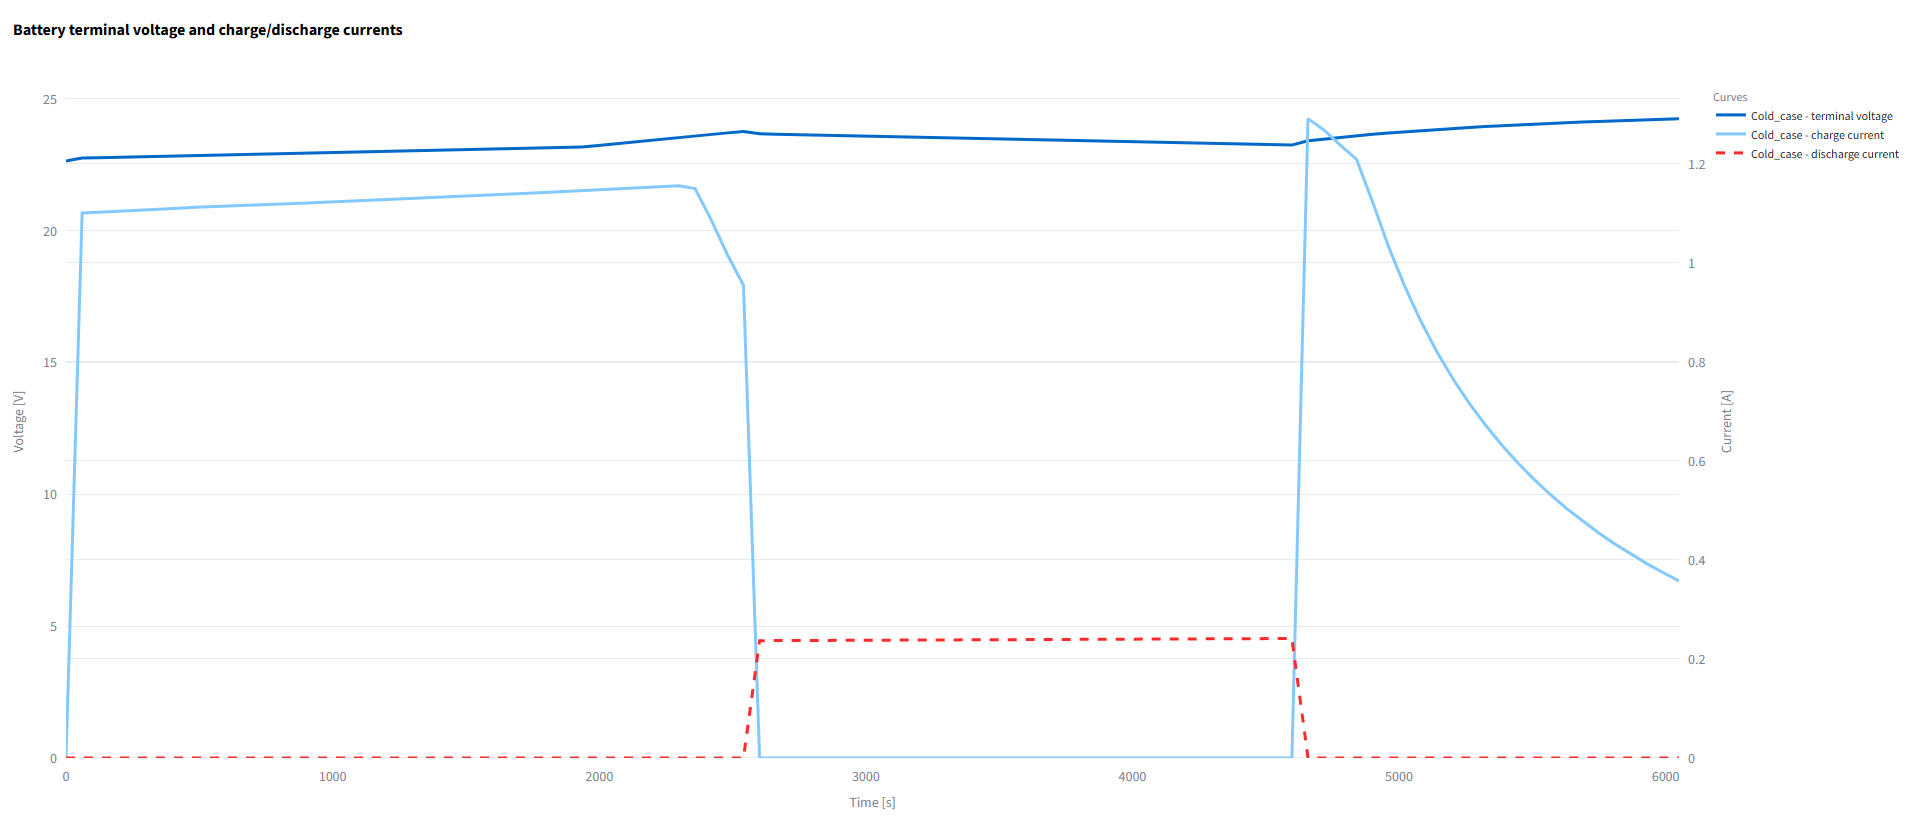
\includegraphics[
            width=\textwidth,
            keepaspectratio
        ]{Figures/09/cold_battery_voltage_current.png}
        \caption{Cold case.}
        \label{fig:cold_battery_voltage_current_ch9}
    \end{subfigure}

    \caption{Battery terminal voltage and charge/discharge currents for the
    nominal, hot and cold transient cases.}
    \label{fig:battery_voltage_current_comparison}    
\end{figure}

\FloatBarrier

% File: Tables/table_multicase_battery_summary.tex
% Usage: \MultiCaseBatterySummaryTable[0.86\textwidth]
% Values obtained from the joint battery-summary export.

\newcommand{\MultiCaseBatterySummaryTable}[1][0.86\textwidth]{%
\begin{table}[H]
    \centering
    \caption{Main battery results for the nominal, hot and cold transient
    cases using the common battery configuration.}
    \label{tab:multicase_battery_summary}
    \footnotesize
    \renewcommand{\arraystretch}{1.30}
    \setlength{\tabcolsep}{4.8pt}
    \begin{tabularx}{#1}{
        |>{\raggedright\arraybackslash}X
        |>{\centering\arraybackslash}c
        |>{\centering\arraybackslash}c
        |>{\centering\arraybackslash}c
        |>{\centering\arraybackslash}c|
    }
        \hline
        \textbf{Result} &
        \textbf{Nominal} &
        \textbf{Hot} &
        \textbf{Cold} &
        \textbf{Unit} \\ \hline
        Final state of charge
        & 95.98 & 93.87 & 93.75 & \% \\ \hline
        Minimum state of charge
        & 60.00 & 60.00 & 60.00 & \% \\ \hline
        Maximum state of charge
        & 95.98 & 97.56 & 93.75 & \% \\ \hline
        Maximum charge power
        & 35.39 & 35.40 & 30.42 & W \\ \hline
        Maximum discharge power
        & 11.22 & 16.84 & 3.06 & W \\ \hline
        Battery-temperature range
        & 18.40--20.90 & 35.50--38.20 & 3.66--4.46 & $^\circ$C \\ \hline
        Minimum charge-derating factor
        & 1.000 & 1.000 & 0.733 & -- \\ \hline
        Charge-derated duration
        & 0.00 & 0.00 & 100.84 & min \\ \hline
        Curtailed solar energy
        & 282.51 & 368.19 & 275.99 & Wh \\ \hline
        Unserved-load energy
        & $\approx 0$ & $\approx 0$ & $\approx 0$ & Wh \\ \hline
    \end{tabularx}
\end{table}%
}
\MultiCaseBatterySummaryTable[0.7\textwidth]

The nominal voltage ranges from $22.65$ to $24.38\,\mathrm{V}$, with maximum
charge and discharge currents of $1.50$ and $0.95\,\mathrm{A}$. The hot case
reaches $24.52\,\mathrm{V}$ and the largest discharge current,
$1.30\,\mathrm{A}$, consistently with its $30.87\,\mathrm{W}$ maximum
discharge power. The cold case reaches $24.25\,\mathrm{V}$, while its maximum
charge and discharge currents remain at $1.29$ and $0.24\,\mathrm{A}$. The
reduced cold-case current is consistent with both the lower selected load and
the active charge derating.

The summary confirms that no case reaches the lower SOC limit or leaves
electrical demand unserved. The hot case produces the largest curtailed solar
energy, $364.18\,\mathrm{Wh}$, because its high generation frequently exceeds
the power and current accepted by the battery. The nominal and cold values are
similar, $276.23$ and $274.51\,\mathrm{Wh}$, although the physical causes
differ: the nominal battery is unrestricted thermally, while the cold battery
rejects additional surplus because of its reduced charge capability.


\section{Overall Comparison}
\label{sec:overall_comparison}

The selected cases provide the expected upper and lower thermal environments
without changing the common model architecture. The hot case produces the
highest equipment temperatures and the largest OBC--radiator interface
difference, while the cold case produces the lowest temperatures and activates
the battery charge derating. The nominal solution generally remains between
both limits, although differences in eclipse timing can temporarily reverse
the ordering of solar-panel temperatures, loads and heat flows.

The transient comparisons also show that absolute temperature, temporal
variation and spatial non-uniformity are separate results. The hot case has the
highest temperatures but the smallest $30\,\mathrm{min}$ variation of
\texttt{BODY\_PANEL}; the cold battery has the lowest temperature but also the
smallest internal battery range. Interface and flow results similarly depend
on the local connection and can change node pair, magnitude or direction
between cases.

The electrical response is governed by both illumination and temperature.
Higher panel temperature reduces instantaneous conversion efficiency, whereas
eclipse duration controls the total generated energy and the discharge
interval. The hot case consequently generates the most energy but ends with
the lowest final SOC because its high load and late eclipse produce the
strongest discharge near the end of the simulation. The cold case receives
the least solar energy and remains thermally derated, but its reduced demand
prevents unserved load and allows the battery to finish above $93\%$ SOC.

The combined results confirm the value of retaining both superposed curves and
\textit{Case difference}. Absolute representations preserve the operating
levels required to assess temperatures, flows and battery limits, while the
difference mode quantifies the separation from the nominal solution and makes
the influence of non-coincident orbital events directly visible.

\FloatBarrier
